\documentclass{homework}
\newcommand{\R}{\textbf{R}}
\newcommand{\dee}{\;\text{d}}
\newcommand{\eps}{\varepsilon}
\newcommand{\pl}[2]{\frac{\partial #1}{\partial #2}}
\newcommand{\dl}[2]{\frac{\text{d} #1}{\text{d} #2}}
\newcommand{\sgn}{\text{sgn}}
\newcommand{\bigoh}{\mathcal{O}}
\usepackage{enumitem}

\newcommand{\hwclass}{Math 6108}
\newcommand{\hwname}{Jacob Hauck}
\newcommand{\hwtype}{Homework}


\usepackage{listings}
\usepackage{booktabs}
\usepackage{subcaption}

\newcommand{\hwnum}{8}
\renewcommand{\questiontype}{Problem}

\begin{document}
	\maketitle
	
	\question Consider the BVP
	\begin{alignat*}{2}
		\Delta u &= -2\pi^2\sin(\pi(x+y)) = f(x,y), &\qquad &0<x<1, \quad 0<y<1 \\
		u(0,y) &= \sin(\pi y) = g_\ell(y), \quad u(1, y) = \sin(\pi(1+y)) = g_r(y), & \qquad &0 \le y \le 1\\
		u(x,0) &= \sin(\pi x) = g_b(x), \quad u(x, 1) = \sin(\pi(1+x)) = g_t(x), & \qquad &0 \le x \le 1. 
	\end{alignat*}
	The exact solution of this equation is given by $u(x,y) = \sin(\pi(x+y))$.
	
	\begin{alphaparts}
		\questionpart Consider a grid of sample points $\{(x_i, y_j)\}$ on the domain $[0,1]^2$, where $i = 0,1,\dots, M$, and $j = 0,1,\dots, N$. If the points are evenly spaced horizontally by $h_x = \frac{1}{M}$ and vertically by $h_y = \frac{1}{N}$, then $x_i = ih_x$, and $y_j = jh_y$.
		
		We approximate $u(x_i,y_j)$ by $u_{i,j}$. Using a centered-difference scheme to approximate $\Delta u$ on the interior and applying the boundary conditions on the boundary points, we are led to the numerical scheme
		\begin{equation*}
			\tag{$i,j$}
			\begin{split}
				\frac{u_{i-1,j} - 2u_{i,j} + u_{i+1,j}}{h_x^2} + \frac{u_{i,j-1} -2 u_{i,j} + u_{i,j+1}}{h_y^2} = f(x_i, y_i),\\  i=1,2,\dots, M-1,\; j=1,2,\dots N-1,
			\end{split}
		\end{equation*}
		and
		\begin{alignat*}{3}
			u_{0,j} &= g_\ell(y_j),& \qquad u_{M,j} &= g_r(y_j),& \qquad j&=0,1,\dots,N,\\
			u_{i,0} &= g_b(x_i), & \qquad u_{i,N} &= g_t(x_i),& \qquad i&=0,1,\dots M.
		\end{alignat*}
		
		In order to solve this linear system, we need to reshape the matrix of unknowns $\{u_{i,j}\}_{i=1,j=1}^{M-1,N-1}$ into a vector $U$ and rewrite the corresponding equations $(i,j)$ as a matrix-vector system, substituting the known boundary values where applicable.
		
		We use row-wise ordering to reshape the matrix of unknowns; that is, we define the block vector of rows of the unknown matrix
		\begin{equation*}
			U = \left[\begin{matrix}U^{(1)} \\ U^{(2)} \\ \vdots \\ U^{(N-1)}\end{matrix}\right], \qquad U^{(j)} = \left[\begin{matrix}u_{1,j} \\ u_{2,j} \\ \vdots \\ u_{M-1,j}\end{matrix}\right], \quad j =1,2,\dots, N-1.
		\end{equation*}
		We can rewrite the equations $(i,j)$ into a matrix-vector system, expressing the matrix $A$ and vector $b$ in block form corresponding to the blocks of $U$:
		\begin{equation*}
			A = \left[\begin{matrix}A^{(1,1)} &\hdots& A^{(1,N-1)} \\\vdots &\ddots & \vdots \\ A^{(N-1,1)} & \hdots & A^{(N-1,N-1)}\end{matrix}\right], \qquad b = \left[\begin{matrix}b^{(1)} \\ b^{(2)} \\ \vdots \\ b^{(N-1)}\end{matrix}\right].
		\end{equation*}
		We remark that the block $A^{(j,j')}$ expresses the dependence of equations $(1,j), (2,j), \dots, (M-1,j)$ on the unknowns in row $j'$ of the unknown matrix $\{u_{i,j}\}$. 
		
		We construct $A$ and $b$ one block row at a time. Consider the blocks $A^{(1,j')}$ for $j'=1,2,\dots, N-1$, the first row of blocks of $A$. As mentioned, these blocks correspond to equations $(1,1),(2,1), \dots, (M-1,1)$. Substituting in boundary conditions, we see that
		\begin{align*}
			(1,1) &\implies \left(-\frac{2}{h_x^2}-\frac{2}{h_y^2}\right)u_{1,1} + \frac{1}{h_x^2}u_{2,1} + \frac{1}{h_y^2}u_{1,2} = f(x_1,y_1) - \frac{g_\ell(y_1)}{h_x^2} - \frac{g_b(x_1)}{h_y^2} \\
			\substack{(i,1) \\ i=2,\dots,M-2} &\implies \left(-\frac{2}{h_x^2}-\frac{2}{h_y^2}\right)u_{i,1} + \frac{1}{h_x^2}u_{i-1,1} + \frac{1}{h_x^2}u_{i+1,1} + \frac{1}{h_y^2}u_{i,2} = f(x_i,y_1) - \frac{g_b(x_i)}{h_y^2} \\
			(M-1,1) &\implies \left(-\frac{2}{h_x^2}-\frac{2}{h_y^2}\right)u_{M-1,1} + \frac{1}{h_x^2}u_{M-2,1} + \frac{1}{h_y^2}u_{M-1,2} = f(x_{M-1}, y_1) - \frac{g_r(y_1)}{h_x^2} - \frac{g_b(x_{M-1})}{h_y^2}.
		\end{align*}
		Thus, each equation depends only on rows 1 and 2 of the matrix $\{u_{i,j}\}$, so only blocks $A^{(1,1)}$ and $A^{(1,2)}$ are nonzero. Examining these dependencies, we get
		\begin{equation*}
			A^{(1,1)} = \left[\begin{matrix}
				-\frac{2}{h_x^2}-\frac{2}{h_y^2} & \frac{1}{h_x^2} \\
				\frac{1}{h_x^2} & -\frac{2}{h_x^2}-\frac{2}{h_y^2} & \frac{1}{h_x^2} \\
				& & \ddots \\
				& & \frac{1}{h_x^2} & -\frac{2}{h_x^2}-\frac{2}{h_y^2}
			\end{matrix}\right], \qquad
			A^{(1,2)} = \left[\begin{matrix}\frac{1}{h_y^2} \\ & \ddots \\ & & \frac{1}{h_y^2} \end{matrix}\right],
		\end{equation*}
		where blanks indicate zero entries. The block $b^{(1)}$ corresponding to the right hand sides of equations $(1,1),(2,1), \dots, (M-1,1)$ we can read off easily:
		\begin{equation*}
			b^{(1)} = \left[\begin{matrix}
				f(x_1,y_1) - \frac{g_\ell(y_1)}{h_x^2} - \frac{g_b(x_1)}{h_y^2} \\
				f(x_2,y_1) - \frac{g_b(x_2)}{h_y^2} \\
				f(x_3,y_1) - \frac{g_b(x_3)}{h_y^2} \\
				\vdots \\
				f(x_{M-2}, y_1) - \frac{g_b(x_{M-2})}{h_y^2} \\
				f(x_{M-1}, y_1) - \frac{g_r(y_1)}{h_x^2} - \frac{g_b(x_{M-1})}{h_y^2}
			\end{matrix}\right].
		\end{equation*}
		Now consider the blocks $A^{(j,j')}$ for $j = 2,3,\dots, N-2$, and $j' = 1,2,\dots, N-1$. These correspond to equations $(1,j),(2,j),\dots,(M-1,j)$. Substituting boundary conditions, we have
		\begin{align*}
			(1,j) &\implies \left(-\frac{2}{h_x^2}-\frac{2}{h_y^2}\right)u_{1,j} + \frac{1}{h_x^2}u_{2,j} + \frac{1}{h_y^2}u_{1,j-1} + \frac{1}{h_y^2}u_{1,j+1} = f(x_1,y_j) - \frac{g_\ell(y_j)}{h_x^2} \\
			\substack{(i,j) \\ i=2,\dots,M-2} &\implies \left(-\frac{2}{h_x^2}-\frac{2}{h_y^2}\right)u_{i,j} + \frac{1}{h_x^2}u_{i-1,j} + \frac{1}{h_x^2}u_{i+1,j} + \frac{1}{h_y^2}u_{i,j-1} + \frac{1}{h_y^2}u_{i,j+1} = f(x_i,y_j) \\
			(M-1,j) &\implies \left(-\frac{2}{h_x^2}-\frac{2}{h_y^2}\right)u_{M-1,j} + \frac{1}{h_x^2}u_{M-2,j} + \frac{1}{h_y^2}u_{M-1,j-1} + \frac{1}{h_y^2}u_{M-1,j+1} = f(x_{M-1}, y_j) - \frac{g_r(y_j)}{h_x^2}.
		\end{align*}
		Thus, each equation depends only on rows $j-1$, $j$, and $j+1$ of the matrix $\{u_{i,j}\}$, so only blocks $A^{(j,j-1)}$, $A^{(j,j)}$, and $A^{(j,j+1)}$ are nonzero. Examining these dependencies gives
		\begin{equation*}
			A^{(j,j)} = \left[\begin{matrix}
				-\frac{2}{h_x^2}- \frac{2}{h_y^2} & \frac{1}{h_x^2} \\
				\frac{1}{h_x^2} & -\frac{2}{h_x^2} - \frac{2}{h_y^2} & \frac{1}{h_x^2} \\
				& & \ddots \\
				& & \frac{1}{h_x^2} & -\frac{2}{h_x^2} -\frac{2}{h_y^2}
			\end{matrix}\right],
			\qquad A^{(j,j-1)} = A^{(j,j+1)} = \left[\begin{matrix}\frac{1}{h_y^2} \\ & \ddots \\ &&\frac{1}{h_y^2}\end{matrix}\right].
		\end{equation*}
		The block $b^{(j)}$ can be read off from the right hand sides easily:
		\begin{equation*}
			b^{(j)} = \left[\begin{matrix}
				f(x_1,y_j) - \frac{g_\ell(y_j)}{h_x^2} \\
				f(x_2,y_j) \\
				f(x_3,y_j) \\
				\vdots \\
				f(x_{M-2},y_j) \\
				f(x_{M-1},y_j) - \frac{g_r(y_j)}{h_x^2}
			\end{matrix}\right].
		\end{equation*}
		Finally, consider the blocks $A^{(N-1, j')}$, $j' = 1,2,\dots,N-1$. These correspond to equations $(1,N-1),(2,N-1),\dots,(M-1,N-1)$. Substituting boundary conditions, we have
		\begin{align*}
			(1,N-1) &\implies \left(-\frac{2}{h_x^2}-\frac{2}{h_y^2}\right)u_{1,N-1} + \frac{1}{h_x^2}u_{2,N-1} + \frac{1}{h_y^2}u_{1,N-2} = f(x_1,y_{N-1}) - \frac{g_\ell(y_{N-1})}{h_x^2} - \frac{g_t(x_1)}{h_y^2} \\
			\substack{(i,N-1) \\ i=2,\dots,M-2} &\implies \left(-\frac{2}{h_x^2}-\frac{2}{h_y^2}\right)u_{i,N-1} + \frac{1}{h_x^2}u_{i-1,N-1} + \frac{1}{h_x^2}u_{i+1,N-1} + \frac{1}{h_y^2}u_{i,2} = f(x_i,y_{N-1}) - \frac{g_t(x_i)}{h_y^2} \\
			\begin{split}				
				(M-1,N-1) \implies \left(-\frac{2}{h_x^2}-\frac{2}{h_y^2}\right)u_{M-1,N-1} + \frac{1}{h_x^2}u_{M-2,N-1} + \frac{1}{h_y^2}u_{M-1,N-2} \\= f(x_{M-1}, y_{N-1}) - \frac{g_r(y_{N-1})}{h_x^2} - \frac{g_t(x_{M-1})}{h_y^2}.
			\end{split}
		\end{align*}
		Thus, each equation depends only on rows $N-2$ and $N-1$ of the matrix $\{u_{i,j}\}$, so only blocks $A^{(N-1,N-2)}$ and $A^{(N-1,N-1)}$ are nonzero. Examining these dependencies gives
		\begin{equation*}
			A^{(N-1,N-1)} = \left[\begin{matrix}
				-\frac{2}{h_x^2}- \frac{2}{h_y^2} & \frac{1}{h_x^2} \\
				\frac{1}{h_x^2} & -\frac{2}{h_x^2} - \frac{2}{h_y^2} & \frac{1}{h_x^2} \\
				& & \ddots \\
				& & \frac{1}{h_x^2} & -\frac{2}{h_x^2} -\frac{2}{h_y^2}
			\end{matrix}\right], \qquad
			A^{(N-1,N-2)} = \left[\begin{matrix}\frac{1}{h_y^2} \\ & \ddots \\ &&\frac{1}{h_y^2}\end{matrix}\right].
		\end{equation*}
		The block $b^{(N-1)}$ can be read off from the right hand sides of the equations easily:
		\begin{equation*}
			b^{(N-1)} = \left[\begin{matrix}
				f(x_1,y_{N-1}) - \frac{g_\ell(y_{N-1})}{h_x^2} - \frac{g_t(x_1)}{h_y^2} \\
				f(x_2,y_{N-1}) - \frac{g_t(x_2)}{h_y^2} \\
				f(x_3,y_{N-1}) - \frac{g_t(x_3)}{h_y^2} \\
				\vdots \\
				f(x_{M-2},y_{N-1}) - \frac{g_t(x_{M-2})}{h_y^2}\\
				f(x_{M-1},y_{N-1}) - \frac{g_r(y_{N-1})}{h_x^2} - \frac{g_t(x_{M-1})}{h_y^2}
			\end{matrix}\right].
		\end{equation*}
		Therefore, the entire system of equations $(i,j)$ is equivalent to the matrix-vector equation $AU = b$.
		
		\questionpart See \texttt{problem1.m} for the implementation of the scheme in (a).
		
		\questionpart See Figure \ref{fig:p1c} for the mesh plots of the numerical solution and the error function.
		
		\begin{figure}[h]
			\begin{subfigure}{.45\textwidth}
				\centering
				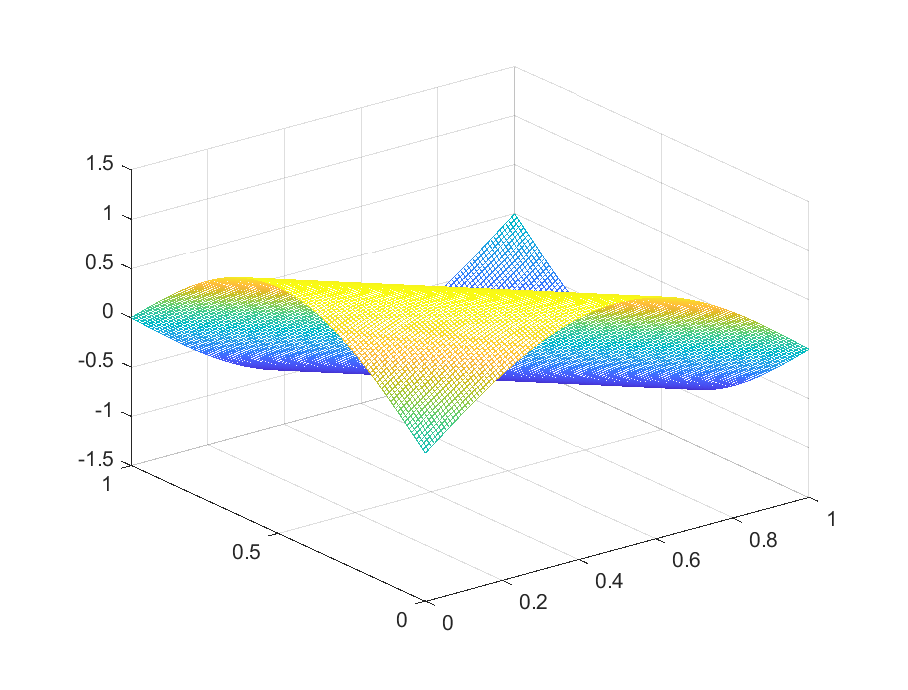
\includegraphics[width=\textwidth]{p1c_u.eps}
				\caption{Numerical solution}
			\end{subfigure}
			\hfill
			\begin{subfigure}{.45\textwidth}
				\centering
				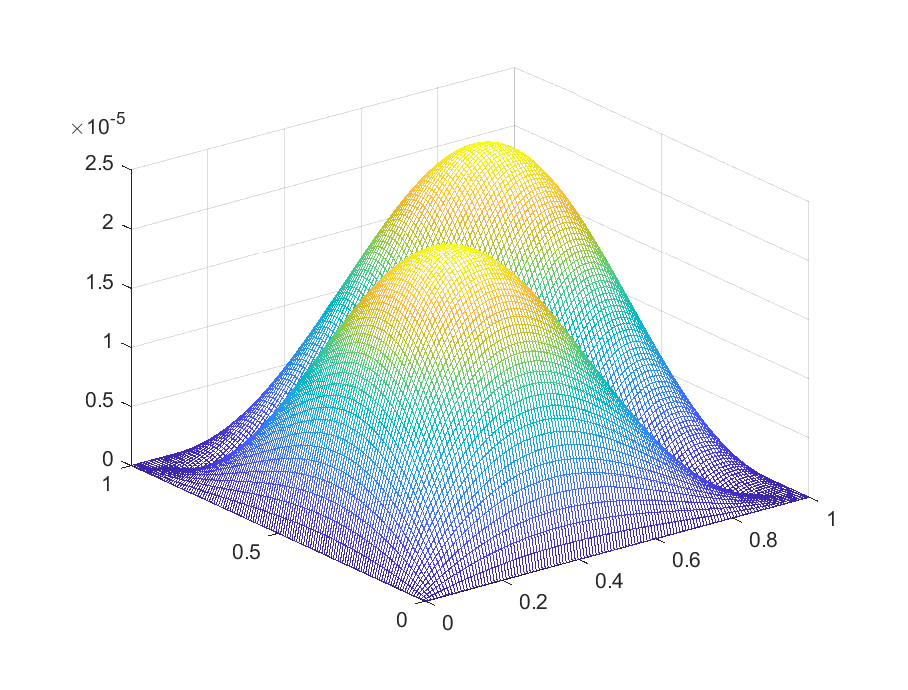
\includegraphics[width=\textwidth]{p1c_error.eps}
				\caption{Numerical error function}
			\end{subfigure}
			\caption{Numerical solution and error function mesh plots with $h_x = h_y=\frac{1}{128}$}
			\label{fig:p1c}
		\end{figure}
		
		\questionpart See Table \ref{table:p1d} for the table of numerical errors and convergence rates for $h = 1/8, 1/16, 1/32, 1/64, 1/128, 1/256$.
		
		\begin{table}[h]
			\centering
			\begin{tabular}{@{}lllll@{}}
				\toprule
				$h$ & $\infty$ error & $\infty$ rate & 2 error & 2 rate \\
				\midrule
				1/8  &	5.992487e-03 &	- &       	2.193459e-03 &	-\\        
				1/16 & 	1.527086e-03 &	1.972373 &	5.495032e-04 &	1.997008 \\
				1/32 & 	3.870626e-04 &	1.980143 &	1.373949e-04 &	1.999799 \\
				1/64  &	9.676442e-05 &	2.000018 &	3.434909e-05 &	1.999985 \\
				1/128  &	2.419921e-05 &	1.999517 &	8.587283e-06 &	1.999998 \\
				1/256  &	6.051066e-06 &	1.999699 &	2.146821e-06 &	2.000000 \\
				\bottomrule
			\end{tabular}
			\caption{Numerical errors and convergence rates for problem 1}
			\label{table:p1d}
		\end{table}
	\end{alphaparts}
	
	\question
	Consider the BVP
	\begin{alignat*}{2}
		\Delta u &= -2\pi^2\sin(\pi x)\sin(\pi y) = f(x,y), &\qquad &0<x<1, \quad 0<y<2 \\
		u(0,y) &= 2 = g_\ell(y), \quad u(1, y) = 2 = g_r(y), & \qquad &0 \le y \le 2\\
		u(x,0) &= 2 = g_b(x), \quad u(x, 1) = 2 = g_t(x), & \qquad &0 \le x \le 1. 
	\end{alignat*}
	The exact solution of this equation is given by $u(x,y) = 2 +\sin(\pi x)\sin(\pi y)$.
	
	\begin{alphaparts}
		\questionpart Consider a grid of sample points $\{(x_i, y_j)\}$ on the domain $[0,1]\times[0,2]$, where $i = 0,1,\dots, M$, and $j = 0,1,\dots, N$. If the points are evenly spaced horizontally by $h_x = \frac{1}{M}$ and vertically by $h_y = \frac{2}{N}$, then $x_i = ih_x$, and $y_j = jh_y$.
		
		We approximate $u(x_i,y_j)$ by $u_{i,j}$. Using a centered-difference scheme to approximate $\Delta u$ on the interior and applying the boundary conditions on the boundary points, we are led to the numerical scheme
		\begin{equation*}
			\tag{$i,j$}
			\begin{split}
				\frac{u_{i-1,j} - 2u_{i,j} + u_{i+1,j}}{h_x^2} + \frac{u_{i,j-1} -2 u_{i,j} + u_{i,j+1}}{h_y^2} = f(x_i, y_i),\\  i=1,2,\dots, M-1,\; j=1,2,\dots N-1,
			\end{split}
		\end{equation*}
		and
		\begin{alignat*}{3}
			u_{0,j} &= g_\ell(y_j),& \qquad u_{M,j} &= g_r(y_j),& \qquad j&=0,1,\dots,N,\\
			u_{i,0} &= g_b(x_i), & \qquad u_{i,N} &= g_t(x_i),& \qquad i&=0,1,\dots M.
		\end{alignat*}
		
		In order to solve this linear system, we need to reshape the matrix of unknowns $\{u_{i,j}\}_{i=1,j=1}^{M-1,N-1}$ into a vector $U$ and rewrite the corresponding equations $(i,j)$ as a matrix-vector system, substituting the known boundary values where applicable.
		
		We use column-wise ordering to reshape the matrix of unknowns; that is, we define the block vector of columns of the unknown matrix
		\begin{equation*}
			U = \left[\begin{matrix}U^{(1)} \\ U^{(2)} \\ \vdots \\ U^{(M-1)}\end{matrix}\right], \qquad U^{(i)} = \left[\begin{matrix}u_{i,1} \\ u_{i,2} \\ \vdots \\ u_{i, N-1}\end{matrix}\right], \quad i =1,2,\dots, M-1.
		\end{equation*}
		We can rewrite the equations $(i,j)$ into a matrix-vector system, expressing the matrix $A$ and vector $b$ in block form corresponding to the blocks of $U$:
		\begin{equation*}
			A = \left[\begin{matrix}A^{(1,1)} &\hdots& A^{(1,M-1)} \\\vdots &\ddots & \vdots \\ A^{(M-1,1)} & \hdots & A^{(M-1,M-1)}\end{matrix}\right], \qquad b = \left[\begin{matrix}b^{(1)} \\ b^{(2)} \\ \vdots \\ b^{(M-1)}\end{matrix}\right].
		\end{equation*}
		We remark that the block $A^{(i,i')}$ expresses the dependence of equations $(i,1), (i,2), \dots, (i, N-1)$ on the unknowns in column $i'$ of the unknown matrix $\{u_{i,j}\}$. 
		
		We construct $A$ and $b$ one block row at a time. Consider the blocks $A^{(1,i')}$ for $i'=1,2,\dots, M-1$, the first row of blocks of $A$. As mentioned, these blocks correspond to equations $(1,1),(1,2), \dots, (1,N-1)$. Substituting in boundary conditions, we see that
		\begin{align*}
			(1,1) &\implies \left(-\frac{2}{h_x^2}-\frac{2}{h_y^2}\right)u_{1,1} + \frac{1}{h_x^2}u_{2,1} + \frac{1}{h_y^2}u_{1,2} = f(x_1,y_1) - \frac{g_\ell(y_1)}{h_x^2} - \frac{g_b(x_1)}{h_y^2} \\
			\substack{(1,j) \\ j=2,\dots,N-2} &\implies \left(-\frac{2}{h_x^2}-\frac{2}{h_y^2}\right)u_{1,j} + \frac{1}{h_x^2}u_{2,j} + \frac{1}{h_y^2}u_{1,j-1} + \frac{1}{h_y^2}u_{1,j+1} = f(x_1,y_j) - \frac{g_\ell(y_j)}{h_x^2}\\
			(1,N-1) &\implies \left(-\frac{2}{h_x^2}-\frac{2}{h_y^2}\right)u_{1,N-1} + \frac{1}{h_x^2}u_{2,N-1} + \frac{1}{h_y^2}u_{1,N-2} = f(x_1, y_{N-1}) - \frac{g_\ell(y_{N-1})}{h_x^2} - \frac{g_t(x_1)}{h_y^2}.
		\end{align*}
		Thus, each equation depends only on columns 1 and 2 of the matrix $\{u_{i,j}\}$, so only blocks $A^{(1,1)}$ and $A^{(1,2)}$ are nonzero. Examining these dependencies, we get
		\begin{equation*}
			A^{(1,1)} = \left[\begin{matrix}
				-\frac{2}{h_x^2}-\frac{2}{h_y^2} & \frac{1}{h_y^2} \\
				\frac{1}{h_y^2} & -\frac{2}{h_x^2}-\frac{2}{h_y^2} & \frac{1}{h_y^2} \\
				& & \ddots \\
				& & \frac{1}{h_y^2} & -\frac{2}{h_x^2}-\frac{2}{h_y^2} 
			\end{matrix}\right], \qquad
			A^{(1,2)} = \left[\begin{matrix}\frac{1}{h_x^2} \\ & \ddots \\ & & \frac{1}{h_x^2} \end{matrix}\right],
		\end{equation*}
		where blanks indicate zero entries. The block $b^{(1)}$ corresponding to the right hand sides of equations $(1,1),(1,2), \dots, (1,N-1)$ we can read off easily:
		\begin{equation*}
			b^{(1)} = \left[\begin{matrix}
				f(x_1,y_1) - \frac{g_\ell(y_1)}{h_x^2} - \frac{g_b(x_1)}{h_y^2} \\
				f(x_1,y_2) - \frac{g_\ell(y_2)}{h_x^2} \\
				f(x_1,y_3) - \frac{g_\ell(y_3)}{h_x^2} \\
				\vdots \\
				f(x_1, y_{N-2}) - \frac{g_\ell(y_{N-2})}{h_x^2} \\
				f(x_1, y_{N-1}) - \frac{g_\ell(y_{N-1})}{h_x^2} - \frac{g_t(x_1)}{h_y^2}
			\end{matrix}\right].
		\end{equation*}
		Now consider the blocks $A^{(i,i')}$ for $i = 2,3,\dots, N-2$, and $i' = 1,2,\dots, N-1$. These correspond to equations $(i,1),(i,2),\dots,(i,N-1)$. Substituting boundary conditions, we have
		\begin{align*}
			(i,1) &\implies \left(-\frac{2}{h_x^2}-\frac{2}{h_y^2}\right)u_{i,1} + \frac{1}{h_x^2}u_{i-1,1} + \frac{1}{h_x^2}u_{i+1,1} + \frac{1}{h_y^2}u_{i,2} = f(x_i,y_1) - \frac{g_b(x_i)}{h_y^2} \\
			\substack{(i,j) \\ j=2,\dots,N-2} &\implies \left(-\frac{2}{h_x^2}-\frac{2}{h_y^2}\right)u_{i,j} + \frac{1}{h_x^2}u_{i-1,j} + \frac{1}{h_x^2}u_{i+1,j} + \frac{1}{h_y^2}u_{i,j-1} + \frac{1}{h_y^2}u_{i,j+1} = f(x_i,y_j) \\
			(i,N-1) &\implies \left(-\frac{2}{h_x^2}-\frac{2}{h_y^2}\right)u_{i,N-1} + \frac{1}{h_x^2}u_{i-1,N-1} + \frac{1}{h_x^2}u_{i+1,N-1} + \frac{1}{h_y^2}u_{i,N-2} = f(x_i, y_{N-1}) - \frac{g_t(x_i)}{h_y^2}.
		\end{align*}
		Thus, each equation depends only on columns $i-1$, $i$, and $i+1$ of the matrix $\{u_{i,j}\}$, so only blocks $A^{(i,i-1)}$, $A^{(i,i)}$, and $A^{(i,i+1)}$ are nonzero. Examining these dependencies gives
		\begin{equation*}
			A^{(i,i)} = \left[\begin{matrix}
				-\frac{2}{h_x^2}- \frac{2}{h_y^2} & \frac{1}{h_y^2} \\
				\frac{1}{h_y^2} & -\frac{2}{h_x^2} - \frac{2}{h_y^2} & \frac{1}{h_y^2} \\
				& & \ddots \\
				& & \frac{1}{h_y^2} & -\frac{2}{h_x^2} -\frac{2}{h_y^2}
			\end{matrix}\right],
			\qquad A^{(i,i-1)} = A^{(i,i+1)} = \left[\begin{matrix}\frac{1}{h_x^2} \\ & \ddots \\ &&\frac{1}{h_x^2}\end{matrix}\right].
		\end{equation*}
		The block $b^{(i)}$ can be read off from the right hand sides easily:
		\begin{equation*}
			b^{(i)} = \left[\begin{matrix}
				f(x_i,y_1) - \frac{g_b(x_i)}{h_y^2} \\
				f(x_i,y_2) \\
				f(x_i,y_3) \\
				\vdots \\
				f(x_i,y_{N-2}) \\
				f(x_i,y_{N-1}) - \frac{g_t(x_i)}{h_y^2}
			\end{matrix}\right].
		\end{equation*}
		Finally, consider the blocks $A^{(M-1, i')}$, $i' = 1,2,\dots,M-1$. These correspond to equations $(M-1,1),(M-1,2),\dots,(M-1,N-1)$. Substituting boundary conditions, we have
		\begin{align*}
			(M-1,1) &\implies \left(-\frac{2}{h_x^2}-\frac{2}{h_y^2}\right)u_{M-1,1} + \frac{1}{h_x^2}u_{M-2,1} + \frac{1}{h_y^2}u_{M-1,2} = f(x_1,y_{N-1}) - \frac{g_r(y_1)}{h_x^2} - \frac{g_b(x_{M-1})}{h_y^2} \\
			\substack{(M-1,j) \\ j=2,\dots,N-2} &\implies \left(-\frac{2}{h_x^2}-\frac{2}{h_y^2}\right)u_{M-1,j} + \frac{1}{h_x^2}u_{M-2,j} + \frac{1}{h_y^2}u_{M-1,j-1} + \frac{1}{h_y^2}u_{M-1,j+1} = f(x_{M-1},y_j) - \frac{g_r(y_j)}{h_x^2} \\
			\begin{split}				
				(M-1,N-1) \implies \left(-\frac{2}{h_x^2}-\frac{2}{h_y^2}\right)u_{M-1,N-1} + \frac{1}{h_x^2}u_{M-2,N-1} + \frac{1}{h_y^2}u_{M-1,N-2} \\= f(x_{M-1}, y_{N-1}) - \frac{g_r(y_{N-1})}{h_x^2} - \frac{g_t(x_{M-1})}{h_y^2}.
			\end{split}
		\end{align*}
		Thus, each equation depends only on columns $M-2$ and $M-1$ of the matrix $\{u_{i,j}\}$, so only blocks $A^{(M-1,M-2)}$ and $A^{(M-1,M-1)}$ are nonzero. Examining these dependencies gives
		\begin{equation*}
			A^{(N-1,N-1)} = \left[\begin{matrix}
				-\frac{2}{h_x^2}- \frac{2}{h_y^2} & \frac{1}{h_y^2} \\
				\frac{1}{h_y^2} & -\frac{2}{h_x^2} - \frac{2}{h_y^2} & \frac{1}{h_y^2} \\
				& & \ddots \\
				& & \frac{1}{h_y^2} & -\frac{2}{h_x^2} -\frac{2}{h_y^2}
			\end{matrix}\right], \qquad
			A^{(N-1,N-2)} = \left[\begin{matrix}\frac{1}{h_x^2} \\ & \ddots \\ &&\frac{1}{h_x^2}\end{matrix}\right].
		\end{equation*}
		The block $b^{(M-1)}$ can be read off from the right hand sides of the equations easily:
		\begin{equation*}
			b^{(M-1)} = \left[\begin{matrix}
				f(x_{M-1},y_1) - \frac{g_r(y_1)}{h_x^2} - \frac{g_b(x_{M-1})}{h_y^2} \\
				f(x_{M-1},y_2) - \frac{g_r(y_2)}{h_x^2} \\
				f(x_{M-1},y_3) - \frac{g_r(y_3)}{h_x^2} \\
				\vdots \\
				f(x_{M-1},y_{N-2}) - \frac{g_r(y_{N-2})}{h_x^2}\\
				f(x_{M-1},y_{N-1}) - \frac{g_r(y_{N-1})}{h_x^2} - \frac{g_t(x_{M-1})}{h_y^2}
			\end{matrix}\right].
		\end{equation*}
		Therefore, the entire system of equations $(i,j)$ is equivalent to the matrix-vector equation $AU = b$.
		
		\questionpart See \texttt{problem2.m} for the implementation of the scheme in (a).
		
		
		
		\questionpart See Figure \ref{fig:p2c} for the mesh plots of the numerical solution and the error function.
		
		\begin{figure}[h]
			\begin{subfigure}{.45\textwidth}
				\centering
				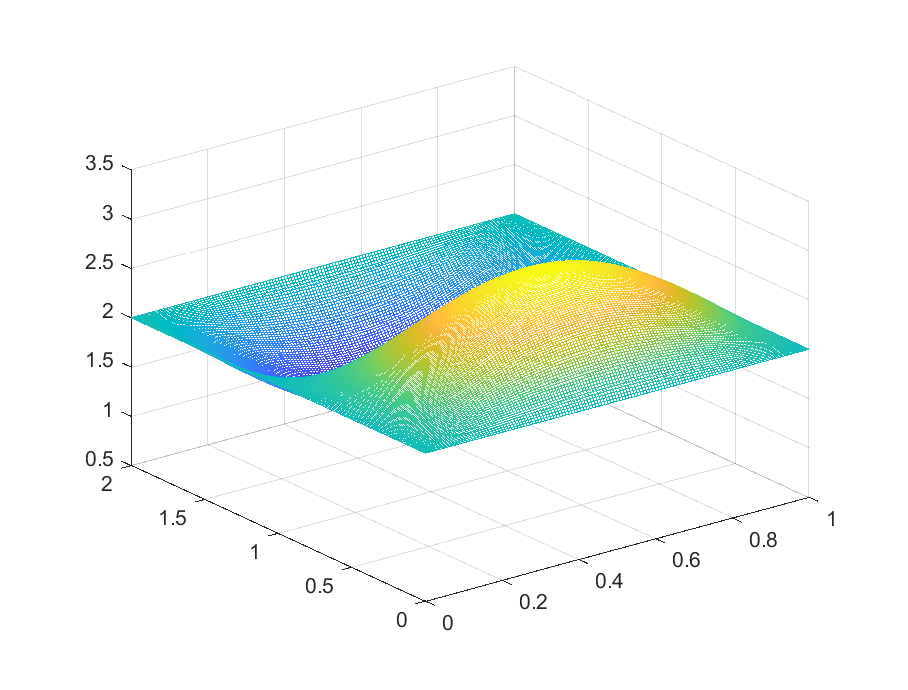
\includegraphics[width=\textwidth]{p2c_u.eps}
				\caption{Numerical solution}
			\end{subfigure}
			\hfill
			\begin{subfigure}{.45\textwidth}
				\centering
				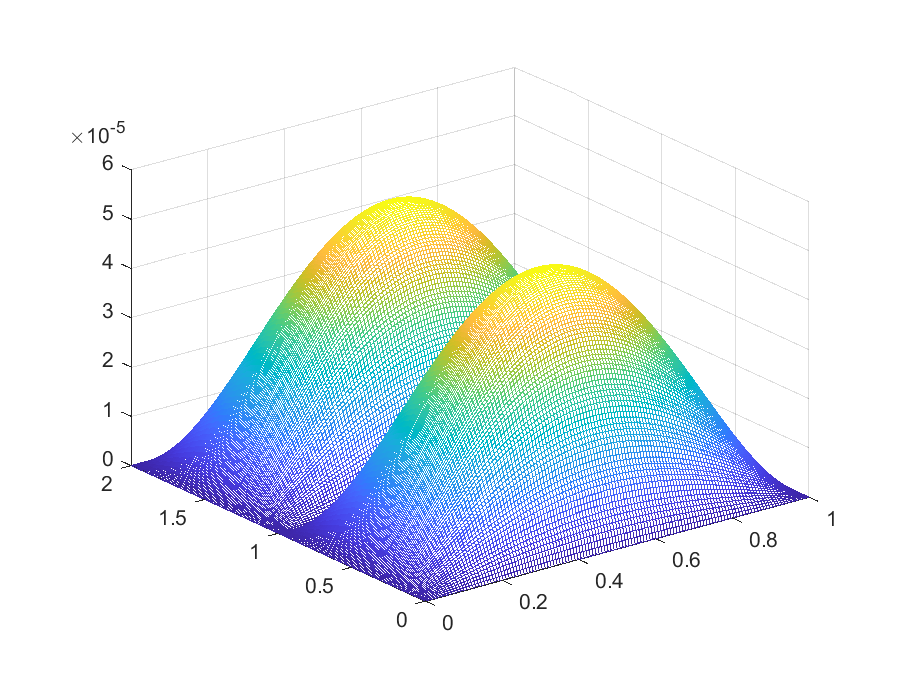
\includegraphics[width=\textwidth]{p2c_error.eps}
				\caption{Numerical error function}
			\end{subfigure}
			\caption{Numerical solution and error function mesh plots with $h_x = h_y=\frac{1}{128}$}
			\label{fig:p2c}
		\end{figure}
		
		\questionpart See Table \ref{table:p2d} for the table of numerical errors and convergence rates for $h = 1/8, 1/16, 1/32, 1/64, 1/128, 1/256$.
		
		\begin{table}[h]
			\centering
			\begin{tabular}{@{}lllll@{}}
				\toprule
				$h$ & $\infty$ error & $\infty$ rate & 2 error & 2 rate \\
				\midrule
				1/8 & 	1.295075e-02&	-        &	9.157561e-03&	- \\
				1/16 & 	3.218964e-03&	2.008367&	2.276152e-03&	2.008367 \\
				1/32  &	8.035777e-04&	2.002087&	5.682152e-04&	2.002087 \\
				1/64  &	2.008218e-04&	2.000522&	1.420025e-04&	2.000522 \\
				1/128  &5.020092e-05&	2.000130&	3.549741e-05&	2.000130 \\
				1/256  &1.254995e-05&	2.000032&	8.874152e-06&	2.000033 \\
				\bottomrule
			\end{tabular}
			\caption{Numerical errors and convergence rates for problem 2}
			\label{table:p2d}
		\end{table}
	\end{alphaparts}
	
	\question Consider the BVP
	\begin{alignat*}{2}
		\Delta u &= -2\pi^2\sin(\pi(x+y)) = f(x,y), &\qquad &0<x<1, \quad 0<y<1 \\
		u(0,y) &= \sin(\pi y) = g_\ell(y), \quad u_x(1, y) = \pi\cos(\pi(1+y)) = g_r(y), & \qquad &0 \le y \le 1\\
		u_y(x,0) &= \pi\cos(\pi x) = g_b(x), \quad u(x, 1) = \sin(\pi(1+x)) = g_t(x), & \qquad &0 \le x \le 1. 
	\end{alignat*}
	The exact solution of this equation is given by $u(x,y) = \sin(\pi(x+y))$.
	
	\begin{alphaparts}
		\questionpart Consider a grid of sample points $\{(x_i, y_j)\}$ on the domain $[0,1]^2$, where $i = 0,1,\dots, M$, and $j = 0,1,\dots, N$. If the points are evenly spaced horizontally by $h_x = \frac{1}{M}$ and vertically by $h_y = \frac{1}{N}$, then $x_i = ih_x$, and $y_j = jh_y$.
		
		We approximate $u(x_i,y_j)$ by $u_{i,j}$. For the Neumann boundary conditions on the right and bottom boundaries, we use a centered difference scheme with ghost points to approximate the derivatives, and extend the PDE to the boundaries to eliminate the ghost points, as follows:
		\begin{equation*}
			\frac{u_{M+1,j} - u_{M-1,j}}{2h_x} = g_r(y_j), \quad j = 1,2,\dots, N-1, \qquad \frac{u_{i,1}-u_{i,-1}}{2h_y} = g_b(x_i), \quad i=1,2,\dots M-1.
		\end{equation*}
		Using a centered-difference scheme to approximate $\Delta u$ on the interior and the points on the parts of the boundary that have a Neumann condition, we obtain the following scheme:
		\begin{equation*}
			\tag{$i,j$}
			\begin{split}
				\frac{u_{i-1,j} - 2u_{i,j} + u_{i+1,j}}{h_x^2} + \frac{u_{i,j-1} -2 u_{i,j} + u_{i,j+1}}{h_y^2} = f(x_i, y_i),\\  i=1,2,\dots, M,\; j=0,2,\dots N-1.
			\end{split}
		\end{equation*}
		For the left and top boundaries, we have Dirichlet boundary conditions, giving
		\begin{equation*}
			u_{0,j} = g_\ell(y_j), \quad j = 0,1,\dots, N, \qquad u_{i,N} = g_t(x_i), \quad i=0,1,\dots, M.
		\end{equation*}
		
		In order to solve this linear system, we need to reshape the matrix of unknowns $\{u_{i,j}\}_{i=1,j=0}^{M,N-1}$ into a vector $U$ and rewrite the corresponding equations $(i,j)$ as a matrix-vector system, substituting the known boundary values and ghost point relationships where applicable.
		
		We use row-wise ordering to reshape the matrix of unknowns; that is, we define the block vector of rows of the unknown matrix
		\begin{equation*}
			U = \left[\begin{matrix}U^{(0)} \\ U^{(1)} \\ \vdots \\ U^{(N-1)}\end{matrix}\right], \qquad U^{(j)} = \left[\begin{matrix}u_{1,j} \\ u_{2,j} \\ \vdots \\ u_{M,j}\end{matrix}\right], \quad j =0,1,\dots, N-1.
		\end{equation*}
		We can rewrite the equations $(i,j)$ into a matrix-vector system, expressing the matrix $A$ and vector $b$ in block form corresponding to the blocks of $U$:
		\begin{equation*}
			A = \left[\begin{matrix}A^{(0,0)} &\hdots& A^{(0,N-1)} \\\vdots &\ddots & \vdots \\ A^{(N-1,0)} & \hdots & A^{(N-1,N-1)}\end{matrix}\right], \qquad b = \left[\begin{matrix}b^{(0)} \\ b^{(1)} \\ \vdots \\ b^{(N-1)}\end{matrix}\right].
		\end{equation*}
		We remark that the block $A^{(j,j')}$ expresses the dependence of equations $(1,j), (2,j), \dots, (M,j)$ on the unknowns in row $j'$ of the unknown matrix $\{u_{i,j}\}$. 
		
		We construct $A$ and $b$ one block row at a time. Consider the blocks $A^{(0,j')}$ for $j'=1,2,\dots, N-1$, the first row of blocks of $A$. As mentioned, these blocks correspond to equations $(1,0),(2,0), \dots, (M,0)$. Substituting in boundary conditions, we see that
		\begin{align*}
			(1,0) &\implies \left(-\frac{2}{h_x^2}-\frac{2}{h_y^2}\right)u_{1,0} + \frac{1}{h_x^2}u_{2,0} + \frac{2}{h_y^2}u_{1,1} = f(x_1,y_0) - \frac{g_\ell(y_0)}{h_x^2} + \frac{2}{h_y}g_b(x_1) \\
			\substack{(i,0) \\ i=2,\dots,M-1} &\implies \left(-\frac{2}{h_x^2}-\frac{2}{h_y^2}\right)u_{i,0} + \frac{1}{h_x^2}u_{i-1,0} + \frac{1}{h_x^2}u_{i+1,0} + \frac{2}{h_y^2}u_{i,1} = f(x_i,y_0) + \frac{2}{h_y}g_b(x_i) \\
			(M,0) &\implies \left(-\frac{2}{h_x^2}-\frac{2}{h_y^2}\right)u_{M,0} + \frac{2}{h_x^2}u_{M-1,0} + \frac{2}{h_y^2}u_{M-1,1} = f(x_{M}, y_0) - \frac{2}{h_x}g_r(y_0) + \frac{2}{h_y}g_b(x_{M}).
		\end{align*}
		Thus, each equation depends only on rows 0 and 1 of the matrix $\{u_{i,j}\}$, so only blocks $A^{(0,0)}$ and $A^{(0,1)}$ are nonzero. Examining these dependencies, we get
		\begin{equation*}
			A^{(1,1)} = \left[\begin{matrix}
				-\frac{2}{h_x^2}-\frac{2}{h_y^2} & \frac{1}{h_x^2} \\
				\frac{1}{h_x^2} & -\frac{2}{h_x^2}-\frac{2}{h_y^2} & \frac{1}{h_x^2} \\
				& & \ddots \\
				& & \frac{2}{h_x^2} & -\frac{2}{h_x^2}-\frac{2}{h_y^2} 
			\end{matrix}\right], \qquad
			A^{(1,2)} = \left[\begin{matrix}\frac{2}{h_y^2} \\ & \ddots \\ & & \frac{2}{h_y^2} \end{matrix}\right],
		\end{equation*}
		where blanks indicate zero entries. The block $b^{(0)}$ corresponding to the right hand sides of equations $(1,0),(2,0), \dots, (M-1,0)$ we can read off easily:
		\begin{equation*}
			b^{(0)} = \left[\begin{matrix}
				f(x_1,y_0) - \frac{g_\ell(y_0)}{h_x^2} + \frac{2}{h_y}g_b(x_1) \\
				f(x_2,y_0) + \frac{2}{h_y}g_b(x_2) \\
				f(x_3,y_0) + \frac{2}{h_y}g_b(x_3) \\
				\vdots \\
				f(x_{M-1}, y_0) +\frac{2}{h_y}g_b(x_{M-1}) \\
				f(x_{M}, y_0) - \frac{2}{h_x}g_r(y_0) + \frac{2}{h_y}g_b(x_M)
			\end{matrix}\right].
		\end{equation*}
		Now consider the blocks $A^{(j,j')}$ for $j = 1,2,3,\dots, N-2$, and $j' = 0,1,\dots, N-1$. These correspond to equations $(1,j),(2,j),\dots,(M,j)$. Substituting boundary conditions, we have
		\begin{align*}
			(1,j) &\implies \left(-\frac{2}{h_x^2}-\frac{2}{h_y^2}\right)u_{1,j} + \frac{1}{h_x^2}u_{2,j} + \frac{1}{h_y^2}u_{1,j-1} + \frac{1}{h_y^2}u_{1,j+1} = f(x_1,y_j) - \frac{g_\ell(y_j)}{h_x^2} \\
			\substack{(i,j) \\ i=2,\dots,M-1} &\implies \left(-\frac{2}{h_x^2}-\frac{2}{h_y^2}\right)u_{i,j} + \frac{1}{h_x^2}u_{i-1,j} + \frac{1}{h_x^2}u_{i+1,j} + \frac{1}{h_y^2}u_{i,j-1} + \frac{1}{h_y^2}u_{i,j+1} = f(x_i,y_j) \\
			(M,j) &\implies \left(-\frac{2}{h_x^2}-\frac{2}{h_y^2}\right)u_{M,j} + \frac{2}{h_x^2}u_{M-1,j} + \frac{1}{h_y^2}u_{M,j-1} + \frac{1}{h_y^2}u_{M,j+1} = f(x_{M}, y_j) - \frac{2}{h_x}g_r(y_j).
		\end{align*}
		Thus, each equation depends only on rows $j-1$, $j$, and $j+1$ of the matrix $\{u_{i,j}\}$, so only blocks $A^{(j,j-1)}$, $A^{(j,j)}$, and $A^{(j,j+1)}$ are nonzero. Examining these dependencies gives
		\begin{equation*}
			A^{(j,j)} = \left[\begin{matrix}
				-\frac{2}{h_x^2}- \frac{2}{h_y^2} & \frac{1}{h_x^2} \\
				\frac{1}{h_x^2} & -\frac{2}{h_x^2} - \frac{2}{h_y^2} & \frac{1}{h_x^2} \\
				& & \ddots \\
				& & \frac{2}{h_x^2} & -\frac{2}{h_x^2} -\frac{2}{h_y^2}
			\end{matrix}\right],
			\qquad A^{(j,j-1)} = A^{(j,j+1)} = \left[\begin{matrix}\frac{1}{h_y^2} \\ & \ddots \\ &&\frac{1}{h_y^2}\end{matrix}\right].
		\end{equation*}
		The block $b^{(j)}$ can be read off from the right hand sides easily:
		\begin{equation*}
			b^{(j)} = \left[\begin{matrix}
				f(x_1,y_j) - \frac{g_\ell(y_j)}{h_x^2} \\
				f(x_2,y_j) \\
				f(x_3,y_j) \\
				\vdots \\
				f(x_{M-1},y_j) \\
				f(x_{M},y_j) - \frac{2}{h_x}g_r(y_j)
			\end{matrix}\right].
		\end{equation*}
		Finally, consider the blocks $A^{(N-1, j')}$, $j' = 0,1,\dots,N-1$. These correspond to equations $(1,N-1),(2,N-1),\dots,(M,N-1)$. Substituting boundary conditions, we have
		\begin{align*}
			(1,N-1) &\implies \left(-\frac{2}{h_x^2}-\frac{2}{h_y^2}\right)u_{1,N-1} + \frac{1}{h_x^2}u_{2,N-1} + \frac{1}{h_y^2}u_{1,N-2} = f(x_1,y_{N-1}) - \frac{g_\ell(y_{N-1})}{h_x^2} - \frac{g_t(x_1)}{h_y^2} \\
			\substack{(i,N-1) \\ i=2,\dots,M-1} &\implies \left(-\frac{2}{h_x^2}-\frac{2}{h_y^2}\right)u_{i,N-1} + \frac{1}{h_x^2}u_{i-1,N-1} + \frac{1}{h_x^2}u_{i+1,N-1} + \frac{1}{h_y^2}u_{i,2} = f(x_i,y_{N-1}) - \frac{g_t(x_i)}{h_y^2} \\
			\begin{split}				
				(M,N-1) \implies \left(-\frac{2}{h_x^2}-\frac{2}{h_y^2}\right)u_{M,N-1} + \frac{2}{h_x^2}u_{M-1,N-1} + \frac{1}{h_y^2}u_{M,N-2} \\= f(x_{M}, y_{N-1}) - \frac{2}{h_x}g_r(y_{N-1}) - \frac{g_t(x_{M})}{h_y^2}.
			\end{split}
		\end{align*}
		Thus, each equation depends only on rows $N-2$ and $N-1$ of the matrix $\{u_{i,j}\}$, so only blocks $A^{(N-1,N-2)}$ and $A^{(N-1,N-1)}$ are nonzero. Examining these dependencies gives
		\begin{equation*}
			A^{(N-1,N-1)} = \left[\begin{matrix}
				-\frac{2}{h_x^2}- \frac{2}{h_y^2} & \frac{1}{h_x^2} \\
				\frac{1}{h_x^2} & -\frac{2}{h_x^2} - \frac{2}{h_y^2} & \frac{1}{h_x^2} \\
				& & \ddots \\
				& & \frac{2}{h_x^2} & -\frac{2}{h_x^2} -\frac{2}{h_y^2}
			\end{matrix}\right], \qquad
			A^{(N-1,N-2)} = \left[\begin{matrix}\frac{1}{h_y^2} \\ & \ddots \\ &&\frac{1}{h_y^2}\end{matrix}\right].
		\end{equation*}
		The block $b^{(N-1)}$ can be read off from the right hand sides of the equations easily:
		\begin{equation*}
			b^{(N-1)} = \left[\begin{matrix}
				f(x_1,y_{N-1}) - \frac{g_\ell(y_{N-1})}{h_x^2} - \frac{g_t(x_1)}{h_y^2} \\
				f(x_2,y_{N-1}) - \frac{g_t(x_2)}{h_y^2} \\
				f(x_3,y_{N-1}) - \frac{g_t(x_3)}{h_y^2} \\
				\vdots \\
				f(x_{M-1},y_{N-1}) - \frac{g_t(x_{M-1})}{h_y^2}\\
				f(x_{M},y_{N-1}) - \frac{2}{h_x}g_r(y_{N-1}) - \frac{g_t(x_{M})}{h_y^2}
			\end{matrix}\right].
		\end{equation*}
		Therefore, the entire system of equations $(i,j)$ is equivalent to the matrix-vector equation $AU = b$.
		
		\questionpart See \texttt{problem3.m} for the implementation of the scheme in (a).
		
		
		
		\questionpart See Figure \ref{fig:p3c} for the mesh plots of the numerical solution and the error function.
		
		\begin{figure}[h]
			\begin{subfigure}{.45\textwidth}
				\centering
				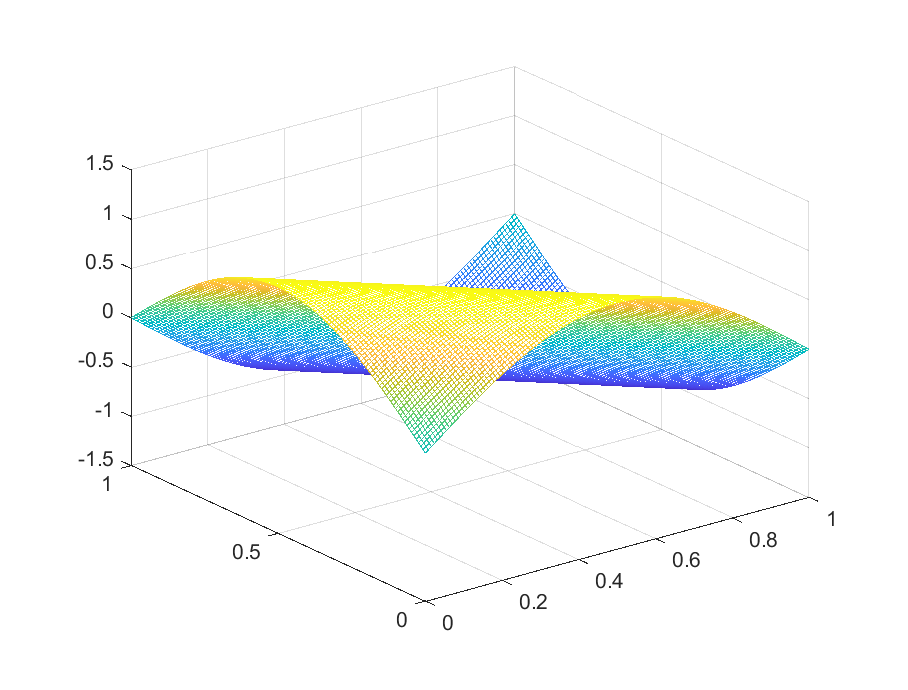
\includegraphics[width=\textwidth]{p3c_u.eps}
				\caption{Numerical solution}
			\end{subfigure}
			\hfill
			\begin{subfigure}{.45\textwidth}
				\centering
				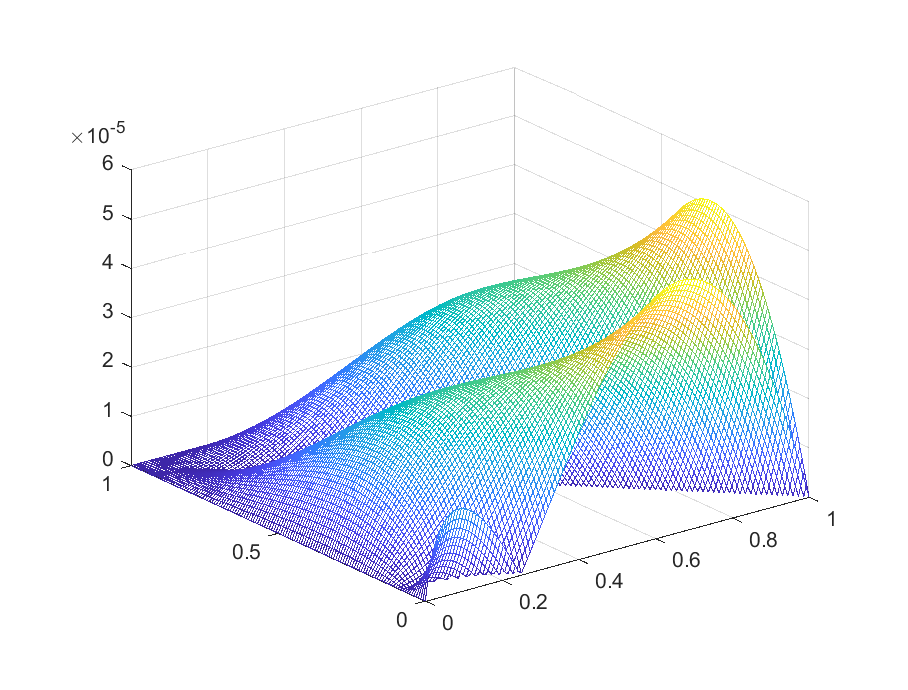
\includegraphics[width=\textwidth]{p3c_error.eps}
				\caption{Numerical error function}
			\end{subfigure}
			\caption{Numerical solution and error function mesh plots with $h_x = h_y=\frac{1}{128}$}
			\label{fig:p3c}
		\end{figure}
		
		\questionpart See Table \ref{table:p3d} for the table of numerical errors and convergence rates for $h = 1/8, 1/16, 1/32, 1/64, 1/128, 1/256$.
		
		\begin{table}[h]
			\centering
			\begin{tabular}{@{}lllll@{}}
				\toprule
				$h$ & $\infty$ error & $\infty$ rate & 2 error & 2 rate \\
				\midrule
				1/8  &	1.296423e-02&	-        &	4.368608e-03&	-        \\
				1/16 & 	3.256417e-03&	1.993179&	1.007073e-03&	2.117006\\
				1/32  &	8.147140e-04&	1.998920&	2.419857e-04&	2.057174\\
				1/64 & 	2.038673e-04&	1.998663&	5.933794e-05&	2.027895\\
				1/128& 	5.096342e-05&	2.000096&	1.469410e-05&	2.013717\\
				1/256& 	1.274146e-05&	1.999932&	3.656267e-06&	2.006794\\
				\bottomrule
			\end{tabular}
			\caption{Numerical errors and convergence rates for problem 3}
			\label{table:p3d}
		\end{table}
	\end{alphaparts}
		
\end{document}